%!TEX root = ../dokumentation.tex

% Spielen Sie Pummelz und formulieren Sie strategische Grundsätze 
% basierend auf Ihren Spielerfahrungen. Basierend auf diesen Spielerfahrungen
% entwerfen Sie ein generelles Vorgehen für Ihre Spiele-KI. Nutzen Sie dazu
% geeignete Konzepte aus der Vorlesung (OODA-Loops, Decision Trees, etc.). 
% Entwerfen Sie ebenfalls eine Architektur in geeigneter Form (UML, FMC 
% oder ähnlich) und dokumentieren Sie sie in Ihrem Entwurfsdokument.
% Das Entwurfsdokument für Aufgabe 1 soll eine maximale Länge von 2-3
% Seiten (mit Abbildungen) haben.

\chapter{Entwurf}

Zu Beginn des Entwurfs wurden sich die folgenden strategischen Grundlagen überlegt. Diese dienen als Grundlage der KI und ihr Handeln in bestimmten Situationen. 

\begin{itemize}
	\item Wenn ein Czaremir (König) im Spiel ist muss sein Überleben jede Runde garantiert werden, da sein Tod das Spiel beendet. Im Gegenzug sollte der gegnerische priorisiert angegriffen werden, um einen schnellen Sieg erzwingen zu können.
	\item Viel hilft viel: in jedem Zug muss mit jeder Figur angegriffen werden die kann. 
	\textbf{Außnahme} sind Angriffe auf:\\
	Bummz wenn er einem selbst mehr Schaden als dem Gegner zufügt\\
	Chilly wenn er nicht \glqq Oneshot\grqq{} ist
	\item Schaden den der Gegner austeilen kann minimieren:
	\begin{itemize}
		\item Schaden auf einen Gegner zu konzentrieren lohnt sich mehr als Schaden auf mehrere Gegner zu verteilen, da so Schaden in der nächsten Runde vermieden werden kann.
		\item Gegner müssen anhand ihrer Eigenschaften klassifiziert werden. Gegner die mehr Schaden austeilen sind früher zu töten, da auch hier Schaden in der nächsten Runde vermieden werden kann
		\item Die KI soll unbedingt die Reichweite der eigenen Einheiten ausnutzen. So soll die Anzahl der gegnerischen Einheiten, die eigene Einheit mit großer Reichweite angreifen kann, gering gehalten werden.
		\item Bummz sich in die Richtung der Gegner und weg von den eigenen Einheiten bewegen.
	\end{itemize}
	\item Einheiten mit geringer Reichweite und hohen Lebenspunkten als \glqq Tanks\grqq{} einsetzen, um andere Einheiten zu schützen.
	\item Einheiten passend gruppieren, sodass Einheiten mit Flächeneffekten (Buffy, Haley) möglichst viele Einheiten um sich stehen haben.
	\item \textbf{ABER:} Aufpassen, dass möglichst viele eigene Einheiten angreifen können, um keine Blockade zu erzeugen und Schaden zu \glqq verlieren\grqq{}
\end{itemize}

Als grundlegendes Konzept soll ein DefaultDecisionTree konzipiert werden, welcher anhand der Spielsituation eine Entscheidung über den Spielzug der jeweiligen Spielfigur trifft. Hierbei wird eine Unterscheidung zwischen einem Angriff und einer Bewegung getroffen. Der Angriffentscheidung liegen drei Abfragen zu Grunde: Kann eine gegnerische Einheit \glqq geoneshotted\grqq{}, getötet oder angegriffen werden. Diese werden in der angegeben Reiehenfolge durchlaufen. Beim Zutreffen des Ereignisses soll dann ein Angriff durchgeführt werden. Die Entscheidung bei mehreren möglichen Einheiten erfolgt über eine festgelegte Hierarchie.

Ein Bewegungszug hat die folgenden beiden Möglichkeiten: Wurden zuvor mehrere Züge ohne einen Angriff vollzogen, so läuft die Einheit aggressiv auf die nächste gegnerische Einheit zu. Ist dies nicht der Fall soll eine Standard-Bewegung ausgeführt werden, bei der die Einheit im besten Fall eine andere angreifen und von keiner gegenerischen Einheit angegriffen werden kann.

\begin{figure}[H]
	\centering
	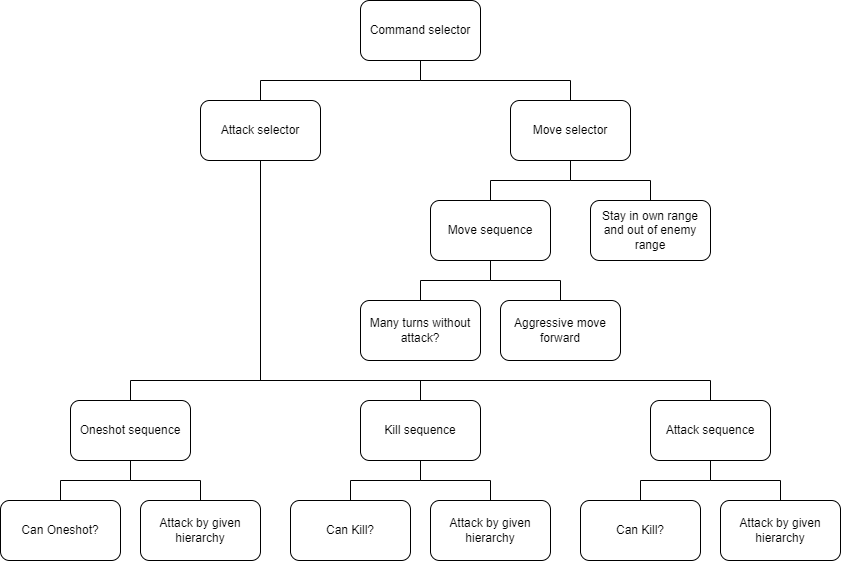
\includegraphics[width=1\linewidth]{konzeptDecisionTree}
	\caption{Konzept eines DecisionTrees zur Pummelz-Command-Entscheidung}
	\label{fig:konzeptDecisionTree}
\end{figure}

Aufbauend auf diesem DefaultDecisionTree sollen weitere DecisionTrees erstellt werden, die auf die Eigenschaften und Spezialfähigkeiten der einzelnen Einheiten zugeschnitten sind und beim Zug der entsprechenden Einheit anstatt des DefaultTrees aufgerufen werden. So ist beispielsweise das Ziel von Bummz von den eigenen Einheiten weg in die gegnerischen zu Rennen. Sneip, Killy und Ängli hingegen sollen sich möglichst weit von gegnerischen Einheiten platzieren, um so wenig möglich Gefahr ausgesetzt zu sein.